\documentclass[]{article}  % list options between brackets
\usepackage{}              % list packages between braces
\usepackage{url}
\usepackage{listings}
\usepackage{graphicx}
\usepackage{color}
\usepackage{enumitem}



% type user-defined commands here

\begin{document}

\title{Real-Time Knowledge Management and Data-mining with Twitter}   % type title between braces
\author{Martin Moghadam, Kalle Grafstr\"{o}m}         % type author(s) between braces
\maketitle

\begin{abstract}
  Real-time tracking of human behavior on Twitter for survey, marketing and analysis. \\     * The research focus (i.e. statement of the problem(s)/research issue(s) addressed);
    * The research methods used (experimental research, case studies, questionnaires, etc.);
    * The results/findings of the research; and
    * The main conclusions and recommendations

\end{abstract}

\section{Introduction}
Knowledge management used to identify and represent insights and experiences gained from data collected from Twitter, can prove useful in many circumstances. Some of which will be discussed in this article, others are left for further development, see discussion section. \\ The validity and credibility of the users identity is not discussed  in detail, we simply assume the user has a valid identity, see references for further details on "The Credibility of Digital Identity Information of the Social Web". \\ The project uses Twitter as a data source to comprise the knowledge, the Tweets all have dates and time allowing use to develop a systems that is updated minute by minute, gathering Information in real-time. This makes it possible to examine a period of time to extract knowledge from the Tweets in that period, for instance a debate performance\cite{bib10}.\\ 

	
\subsection{Twitter}
Twitter is a microblogging and social network service allowing users to send and read small text messages of up to 140 characters. The service has currently more than 100 million users worldwide. Users create accounts with profiles, the basic accounts are provided for free, premium account with a higher number of characters are purchasable. \\ The Tweets are associated to a specific user profile, the profile can have many followers that read the tweets. Each tweets has a time and date information, and can include; profile tags, topic tags and urls , this information can be used to structure and gain a greater understanding of the tweets. \\ The tweets contain different kinds for information as shown in figure \ref{figContent}. 

\begin{figure}[h]
\centering
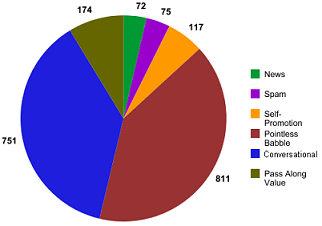
\includegraphics[scale=1]{Content_of_Tweets_Graphed.png}
\caption{Content of Tweets: Source Wikipedia}
\label{figContent}
\end{figure} 
Searching the entire web for this kind of information would yield poor results because of the wast amount of trash data that needs to be sorted though. Such trash data is almost not present in Twitter. People commonly use Twitter to share information of what they are doing and where they are. \\ The knowledge we are interested in, is extracted from the conversational and pass along value data. The data from Twitter is available freely, and there are currently no privacy issues with gathering data.

\subsection{Premise and Usage}
Twitter can and has been used to gather knowledge for:

\begin{itemize}
	\item Real-time recommendations for topical news. \cite{bib5}
	\item Marketing and research.
	\item Disaster monitoring, earthquakes, volcanoes, hurricanes. \cite{bib7}
	\item Political demonstrations. (The Iran demonstrations of 2009)
	\item Counter-terrorism.
	\item Many other possibilities.
\end{itemize}

A few people have used Twitter to make bomb treats, and encouraged assassination of politicians, these treats were not detected or monitored by an application, most of the threats were reported to the authorities by other users of the service and investigated but led to no results, because the threats were not serious just pointless babble. Generally people don't announce acts of terrorism on Twitter, and there has so far been any evidence of a terrorist use Twiiter, making it unsuitable for counter-terrorism.

\section{Knowledge Management}
The knowledge management discipline we work with is social networks analysis, extracting data from the social networks and examining; likes dislikes, friendships, kinship, sexual relationships, beliefs, opinions, and connections to others. The interdependencies can be represented as nodes. \\ These nodes can be graphically represent the data providing a useful structured collection of knowledge. \\  The knowledge can provide a 

\subsection{Real-time Knowledge}

\section{Data Source}
\subsection{Twitter Streams}
\subsection{Real-time Data}
\subsection{Code Example}
\subsection{Test and Development}
       
\section{Discussion}
\subsection{Further Development}

Betweenness, Closeness, Measures in social network analysis
Graphical representation
Node Structuring
Relationship detection
Identity Credibility
Multi-treading and distributed solution for mass real-time Twitter social network analysis


\subsection{Conclusion}

% Creates entry in bibliography even if it isn't cited.
\nocite{bib1} 
\nocite{bib2}
\nocite{bib3}
\nocite{bib4}
\nocite{bib5}
\nocite{bib6}
\nocite{bib7}
\nocite{bib8}
\nocite{bib9}
\nocite{bib10}
\nocite{bib11}
\nocite{bib12}
\nocite{bib13}



\bibliographystyle{unsrt} % references appear in order of citations
\bibliography{references}

\end{document}